%
In diesem Kapitel werden die für Capturing relevante Aspekte  dargestellt. Es
wird dabei analysiert bei welchen Capturing-Komponenten unter welchen Umständen
Engpässe bei der Paketerfassung auftretten können. Anhand der herausgefundenen
Problemen werden Anforderungen und Ansätze für den Entwurf der neuen
Capturing-Software formuliert.  Zu beachten ist, dass die dargestellten Aspekte
sich vollkomen auf die für die Arbeit vorausgesetzten Hardware und Software
beziehen (siehe Abschnitt \ref{sec:hwsw_voraus}).
%
\ifthenelse{\boolean{BRIEF}}{}{
Obwohl die eigentliche Aufgabe der Diplomarbeit in der Analyse und
Verbesserung der Softwarekomponenten liegt, dennoch ist es unentbehrlich ,
die Funktionsweise der darunterliegenden
Hardwarekomponenten zu kennen.  Dies folgt daraus, dass die Hardware die Rolle
eines Betriebsmittels für die Software-Anwendungen spielt, und deshalb
die Software möglichst effektiv die zur Verfügung
gestellte Hardware-Ressourcen nutzen muss. Dafür muss bekannt werden, wie die
einzelne Hardware-Bestandteile funktionieren.

\subsection{Hardwareaspekte bei Capturing}\label{subsec:hw_cap}
% Bla-bla über dem Inhalt dieses Kapitel
In diesem Abschnitt wird die Funktionsweise der Hardware-Komponenten eines
Capturing-Systems vorgestellt. Dabei werden hauptsächlich die für Performance
des Capturing relevanten Aspekte betrachtet.  Und es wird versucht
herauszufinden, welche der Komponenten den
Capturing-Prozess performancemäßig negativ beeinflussen können, und unter welchen
Umständen dies auftritt.

\subsubsection{Netzwerkadapter}\label{sec:adapter}
In diesem Abschnitt wird beschrieben wie der Adapter die Pakete empfängt und
wie er sie in den RAM weiterleitet. Dieses Wissen ist notwendig für die
Auswertung der Capturing-Performance, weil die Engstellen, die auf diesem
ersten Datenweg vorhanden sind, die höhste theoretische Grenze für Performance des gesamten
Capturing-Prozess auf dem Capturing-System bilden. Außerdem, ist die Kenntnis der
Netzwerkadapter-Funktionen auch für das Implementieren der Capturing-Software
unentbehrlich, denn um die Software für den Zugriff auf ankommende Daten
implementieren zu können, muss man zuerst wissen, auf welche Art und Weise die
Hardware diese Daten zur Verfügung stellt.\\\\
%
Außerdem wird in diesem Kapitel das \emph{Interrupt-Coalescing}-Mechanismus des
Intel Gigabit Adapters erläutert. \emph{Interrupt-Coalescing} erlaubt 
die Interrupt-Rate des Adapters zu steuern und damit die Capturing-Performance  zu 
beeinflussen. \\\\
%
% Sagtest Du schon! -- Andi
%Zu beachten, dass die in diesem Abschnitt betrachteten Hardware-Funktionen sich
%vollkommen auf den für die Diplomarbeit vorausgesetzten \textbf{INTEL Pro
%Ethernet Gigabit Adapter} beziehen (siehe Abschnitt \ref{sec:hwsw_voraus}).

\subsubsection*{Paketempfang und DMA-Transfer in RAM}\label{sec:hw_dma} 
Der Empfang eines Paketes an einem Netzwerkadapter schließt das Erkennen des
Paketes auf dem ``wire'', das Anwenden von Adressfilterung, das Speichern des Paketes
auf dem Adapter-Speicher und dann Transfer des Paketes in den RAM ein.  Im RAM
wird pro Paket ein Paket-Puffer alloziert. Die Größe des Paket-Puffers ist
hardwareabhängig und wird durch das Setzen der entsprechenden Bits in
\emph{Receive Control Register} (\verb+RCTL+) des Adapters
festgelegt~\cite{e1000_sdm}. In dem Fall, wenn der Paket größer als der
Paket-Puffer ist, werden mehrere Paket-Puffer für die Speicherung des Paketes
verwendet.\\\\
% DMA. Deskriptor based DMA.
%\reviewnote{Descriptor oder Deskriptor -- eins von Beiden}
Der Datentransport in den RAM wird per DMA (Direct Memory Access) durchgeführt. Es
gibt unterschiedliche DMA-Arten: die ``klassische'' \emph{Register-Based-DMA}
und die \emph{Deskriptor-Based-DMA}~\cite{dma_desc_base}. Der Intel Gigabit
Adapter verwendet die zweite Variante. Beim Deskriptor-Based-DMA werden alle
für DMA benötigte Daten (Ziel-Adresse, Länge des Speichersegments, etc\ldots)
nicht direkt in den DMA-Registern gespeichert, sondern in einem Array im RAM
abgelegt. Jedes Element des Arrays trägt den Namen ``\emph{Deskriptor}''.
Der Deskriptor enthält die Adresse des Puffers im RAM, an die die Daten beim
DMA-Transfer geschrieben werden und andere Bit-Blöcke, die sowohl für die
Steuerung des DMA-Engine des Adapters, als auch zur Benachrichtigung des
Capturing-Prozesses über den Status der DMA-Operation und über Integrität der
empfangenen Daten dienen(siehe Abbildung \ref{dma-e1000-desc}). Für jeden
Puffer im RAM, an den die Daten vom Gerät transferiert werden, bzw. für jeden
DMA-Transfer, steht genau ein Deskriptor zur Verfügung, wobei jeder
Deskriptor nach Abschluss des Transfers erneut für DMA-Transfers
wiederverwendet werden kann.
\begin{figure} 
\centering \includegraphics[width=5.0in]{bilder/Decriptor_e1000}
\caption{DMA-Deskriptor von Intel Ethernet Adapters}
\label{dma-e1000-desc}
\end{figure}
% Intel Pro Deskriptor
\subsubsection*{Deskriptor-Format}\label{sec:deskr_format} 
In Abbildung \ref{dma-e1000-desc} ist das Format des Deskriptors des Intel
Gigabit Adapters dargestellt. Die grau unterlegten Bereiche bezeichnen Felder,
die beim Transfer des Paketes in den RAM, von der Hardware verändert werden.
Wenn der Adapter das Paket aus seinem Adapter-Speicher in den Paket-Puffer im
RAM kopiert, setzt er im entsprechenden Deskriptor die Länge (Length) der in
Puffer gespeicherten Daten, die Prüfsumme (Checksum) des ganzen Paketes, den
Status der DMA-Operation und Fehlerinformationen (Errors) \footnote{Siehe
Software Developer’s Manual~\cite{e1000_sdm}, Seiten: 20-24}.\\\\
%
Die Software kann durch das Lesen der vom Adapter in den Deskriptor
geschriebenen Werte den Zustand des DMA-Transfers und die für das empfangene
Paket relevanten Informationen herausfinden. Außerdem kann die Software auch den
neuen Paket-Puffer allozieren und die Adresse des neuen Puffer im gerade
benutzten Deskriptor setzten, sodass beim nächsten Benutzen des Deskriptor, der
DMA-Transfer in den neuen Puffer stattfindet und die Daten im ``alten''
Paket-Puffer nicht überschreibt.
% Deskriptor-Ring-Array
\subsubsection*{Deskriptor-Ringpuffer}\label{sec:deskr_format} 
Der Adapter betreibt Deskriptoren  als einen Ringpuffer (siehe Abbildung
\ref{img:rdrp}). Der Adapter enthält zwei Register: \emph{Receive Descriptor Head
Register} (RDH) und \emph{Receive Descriptor Tail Register} (RDT), welche die
Rolle von \emph{HEAD-} und \emph{TAIL-}Pointers im Ringpuffer spielen und die
Speicherbereiche mit Deskriptoren referenzieren. Jedes mal, wenn der Adapter ein neues Paket
in den RAM schreibt, wird der Wert im RDH-Register inkrementiert, sodass dieser
Wert dem Deskriptor für den nächsten DMA-Transfer entspricht.  Wenn die
Software die Daten aus dem Paket-Puffer gelesen hat, soll sie den Wert im
RDT-Register inkrementieren, aber so, dass dieser Wert dem Deskriptor entspricht,
der den Paket-Puffer mit dem gerade gelesenen Daten referenziert.
Daraus folgt: 
\begin{itemize}
	\item $RDH = RDT \Longleftrightarrow$ Der Ring ist ``voll'':\\ Es gibt
		keine freien Deskriptoren für einen DMA-Transfer. In diesem Fall stoppt
		die Hardware den Datentransfer in den RAM und wartet bis die Software
		die Pakete in den Paket-Puffern liest (bzw. bearbeitet) und den Wert im
		RDT-Register entsprechend erhöht.
	\item $RDT = (RDH - 1)\ mod\ SIZE \Longleftrightarrow$ Der Ring ist
		``leer'':\\ Die Software hat alle Pakete, die vom Adapter in den RAM
		geschrieben wurden,  bearbeitet und wartet jetzt auf das Ankommen von
		neuen Daten bzw. auf das Erhöhen des Wertes im RDH-Register vom
		Adapter.
\end{itemize}
\begin{figure}
\centering \includegraphics[width=4.0in]{bilder/DescriptorRing}
\caption{Receive Deskriptor Ringpuffer}
\label{img:rdrp}
\end{figure}
% Deskriptor-Array Bild. Beschreibung
In der Abbildung \ref{img:rdrp} ist ein Deskriptor-Ringpuffer dargestellt.  Die
weiss gezeichnete Felder zwischen RDH und RDT, bezeichnen die Deskriptoren, die
für DMA-Transfer der neuen Pakete bereitstehen. Demgegenüber
bezeichnen die graue Felder die Deskriptoren, welche die Paket-Puffer mit den 
neuen Paketen referenzieren, die von der Software noch nicht gelesen wurden.

\subsubsection*{Deskriptor-Fetching}\label{sec:deskr_fetch} 
Um die Werte in den Deskriptoren zu aktualisieren, und um der Software bzw. dem
Adapter die aktualisierten Werte in den Deskriptoren zur Verfügung zu stellen, werden die
Deskriptoren zwischen RAM und Adapter hin- und her kopiert. \\\\
%
Wenn die Software auf den Paket-Puffer mit dem neuen Paket zugegriffen hat,
erhöht sie den Wert im RDT-Register, und stellt damit dem Adapter den
Deskriptor, der den vorher gelesenen Paket-Puffer referenziert, zur Verfügung.
Der Adapter kopiert bei Gelegenheit den Deskriptor in seinen dazu geeigneten
internen Speicher. Und, später, während des  Transfers der aus dem Netz
empfangenen Paketes  in den RAM wird der Deskriptor lokal auf dem Adapter
aktualisiert und wieder zurück in den Deskriptor-Ringpuffer geschrieben.

\subsubsection*{Interrupt}\label{sec:hw_intr}
%\reviewnote{Der letzte Satz hier ist ein fürchterlicher Bandwurmsatz. Mach 3 draus!}
Die Anwesenheit von neuen Paketen im RAM wird vom Adapter durch einen Interrupt
gemeldet.  Die Interrupts, genau gesagt, die Art und Weise, wie die Interrupts
behandelt werden, spielen für die Capturing-Performance eine bedeutende Rolle.
Während der Behandlung eines Adapter-Interrupts sind die Interrupt-Ereignisse
des Adapters gesperrt und das Capturing-System ist nicht mehr in der Lage, das
Ankommen von neuen Paketen zu melden und darauf zu reagieren. Das hat zur
Folge, dass, je länger die Behandlung des Interrupts dauert, die
Wahrscheinlichkeit umso höher ist, dass bevor die Interrupts-Behandlung
abgeschlossen ist, alle freie Paket-Puffer mit neuen Paketen ``gefüllt''
werden. Das führt unvermeidlich zum Verlust der nächsten ankommenden
Pakete.\\\\ 
%
Aus diesem Grund muss die Interrupt-Behandlung-Routine möglichst effizient
implementiert werden und möglichst schnell abgearbeitet werden.
%, um so schnell wie möglich abzuarbeiten, sodass das System
%nicht zu lange im ``Stau'' bleibt und die neue Ereignisse möglichst
%unverzüglich melden und bearbeiten kann, um die Pketverluste zu vermeiden.  
%Die Effizienz der Software 
Die Laufzeit des Interrupt-Handers ist aber noch nicht alles. Wegen des ``Overhead'', den jeder
Interrupt mit sich bringt, spielt auch die Interrupt-Rate eine große Rolle für
Capturing-Performance.\\\\
%
Auf FreeBSD Betriebssystem enthält die Bearbeitung jedes Interrupts 
die folgende Schritte~\cite{freebsd_design}:
%\reviewnote{Was ist ein Hardware-Kontextwechsel??!}
\begin{enumerate}
	\item Hardware und Software Kontextwechsel\footnote{Gemeint ist Umschalten der CPU zwischen Ring-0- und Ring-1-Modus~\cite{pchw} }, die Speicherung von
		CPU-Register, das Wechsel des aktuellen Stack
	\item Zugriff auf die Hardware-Register und Herausfinden der zuständigen
		Interrupt-Service-Routine (ISR)
	\item Aktualisieren der Interrupt-Counters
	\item Ausführen der \emph{Interrupt-Service-Routine}(ISR)
\end{enumerate}
Die Ausführungszeit von ISR (Schritt \textbf{4}) ist variabel und hangt von der
Komplexität der im Interrupt-Kontext ausgeführten Funktionen ab.  Dagegen
bleibt die Ausführungszeit der Schritte \textbf{1} bis \textbf{3}
(eigentlicher Interrupt-Overhead)  konstant und wird bei jeder
Interrupt-Behandlung immer dabei sein.  Die Ausführungszeit der Schritte
\textbf{1} bis \textbf{3} beträgt auf einem konventionellen PC einige
Mikrosekunden~\cite{intrr_coal}, was verursacht, dass bei einer hohe Rate von
Interrupt-Ereignissen (z.B. mehr als $100 000/sec$) ein dominierender Anteil
der CPU-Ressourcen nur für den Interrupt-Overhead verwendet werden kann.
Beim Capturing verursacht das Paket-Verluste.\\\\
%, denn die Anzahl der
%Pakete, die ein Rechnersystem pro ein Zeitintervall empfangen kann, ist
%offensichtlich durch die Anzahl der Pakete, welche die Betriebssystem-Software
%pro diesen Zeitintervall bearbeitet, begrenzt.\\\\
%
Außerdem kann eine hohe Interrupt-Rate das Capturing-System in den
\emph{receive-livelock}-Zustand bringen~\cite{elim_recv_lock}.
\emph{Receive-livelock} ist ein Zustand, in dem das Rechnersystem die ganze
CPU-Zeit lediglich für die Interrupt-Bearbeitung verbraucht und dadurch keine
CPU-Ressourcen für die Ausführung anderer Capturing-Prozesse freigibt. Falls die
Rate der ankommenden Pakete so hoch ist, dass die dadurch enstehende
Interrupt-Load die anderen Prozesse stark vernachlässigt, können 
Paketverluste enstehen, denn die Capturing-Software wird unter FreeBSD sowohl im
Interrupt-Kontext als auch im Userspace ausgeführt.

\subsubsection*{Interrupt-Coalescing}\label{sec:intr_coal}
Zur Beseitigung des receive-livelock-Problems und Minimierung des gesamten
Interrupts-Overhead gibt es die unterschiedliche
Lösungsansätze~\cite{elim_recv_lock, intrr_mod}. Eine davon,
\emph{Interrupt-Coalescing}, wird auf dem Intel Gigabit Adapter verwendet.
Unter dem Begriff Interrupt-Coalescing versteht man das Zusammenfassen von
Interrupts von mehreren Ereignissen zu einem einzigen Interrupts.
%versteckt sich ein Interrupt-Mechanismus
%bei dem jedes Interrupt zur Bearbeitung mehrerer Ereignisse erzeugt werden
%kann. 
In unserem Fall bedeutet dies, dass im Lauf einer Interrupts-Behandlung
nicht nur ein, sondern mehrere empfangene Pakete zusammen bearbeitet werden
können.  Damit lässt sich die Interrupt-Rate reduzieren, was auch zur
Minimierung den gesamten Interrupt-Overhead und gleichzeitig zur Vergrößerung
des Datendurchsatzes bei Capturing führt.\\\\
%
Interrupt-Coalescing wird auf dem Adapter mit Hilfe von drei Timern realisiert~\cite{intrr_mod}:
\begin{description}
	\item[Absolute-Delay-Timer:] Verzögert das Interrupt-Ereignis um ein
		bestimmtes Zeit-Interval (siehe Abbildung \ref{rat}). Der Timer wird nach
		dem Transfer des ersten Paketes in den RAM initialisiert und
		gestartet. Der Timer wird generiert nach dem Ablauf des im
		\verb+RADV+-Register~\cite{e1000_sdm} gesetzten Interval einen Interrupt.
		Nach dem Interrupt, sobald das neue Paket in den RAM
		transferiert wird, wird der Absolute-Timer wieder reinitialisiert und
		gestartet. Der Wert im \verb+RADV+-Register kann durch den
		\emph{sysctl}-Befehl~\cite{man_sysctl} gesetzt werden:
		\begin{equation}
			\verb+# sysctl dev.em.0.rx_abs_int_delay N+
		\end{equation}
%
	\item[Packet-Delay-Timer:] Wie auch der Absolute-Delay-Timer verzögert auch dieser Time
	        nach dem Empfang eines Paketes das Interrupt-Ereignis um ein bestimmtes
		Zeit-Interval (siehe Abbildung \ref{rpt}).  Der Packet-Timer wird aber
		nach jedem Transfer eines neuen Paketes in den RAM jedes mal
		reinitialisiert und wieder gestartet. Der Interrupt des Timers findet
		daher nach Ablauf des Zeit-Intervals nur
		dann statt, wenn während des Zeitintervalls keine neue Pakete vom
		Adapter in den RAM übertragen werden. Das Zeit-Intervall für
		Packet-Timer wird im
		\verb+RDTR+-Register~\cite{e1000_sdm} gesetzt:
		\begin{equation}
			\verb+# sysctl dev.em.0.rx_int_delay N+
		\end{equation}
%
	\item[Interrupt-Throttle-Timer:] Bestimmt eine minimale
		inter-Interrupt-delay für den Adapter. Damit wird  gleichzeitig für
		\emph{receive} und \emph{transmit} eine maximale Interrupt-Rate
		garantiert. Der minimale Zeit-Interval zwischen zwei Interrupts wird in
		\verb+ITR+-Register~\cite{e1000_sdm} gesetzt.\\\\
		%
		Für das Setzen des Wertes in den \verb+ITR+-Register ist kein
		\emph{sysctl} vorgesehen. Um \verb+ITR+ zu setzen, muss man in den Code
		des Treibers über die folgende Makrodefinition die maximale Anzahl der
		Interrupts pro eine Sekunde eingeben: 
		\begin{equation}
			\verb+#define MAX_INTS_PER_SEC        8000+
		\end{equation}
\end{description}
\begin{figure}
\centering \includegraphics[width=4.0in]{bilder/AbsoluteTimer}
\caption{Absolute Delay Timer}
\label{rat}
\end{figure}
%
\begin{figure}
\centering 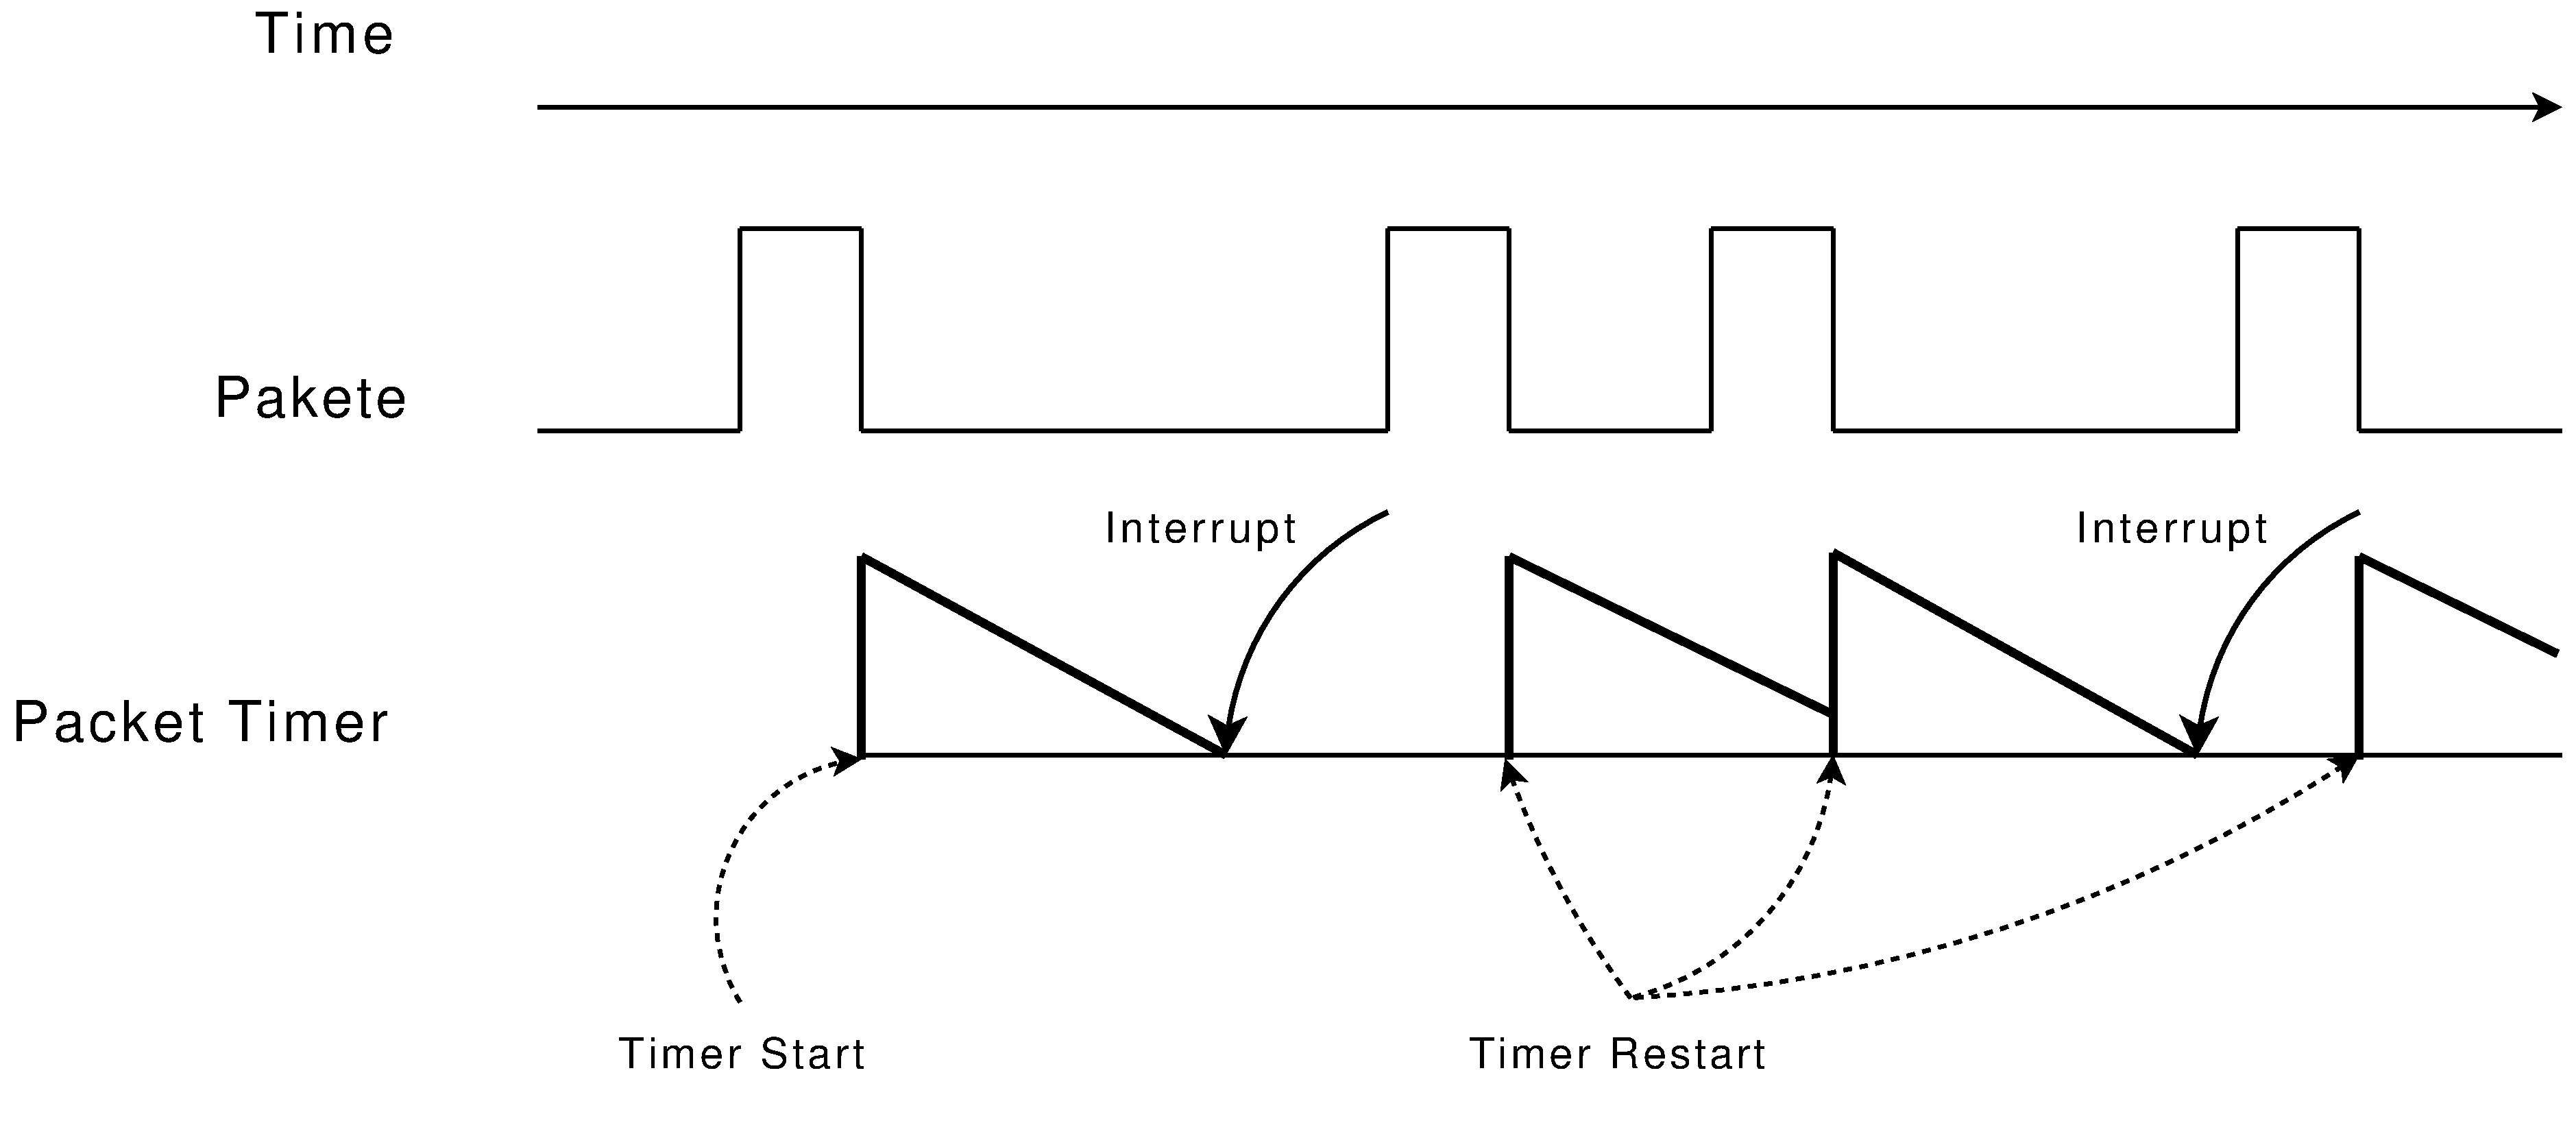
\includegraphics[width=4.0in]{bilder/PacketTimer}
\caption{Packet Delay Timer}
\label{rpt}
\end{figure}
%
Die obengenannten Timer minimieren die Interrupt-Rate durch Verzögerung der
Interrupt-Ereignisse. Bei einer hohen ständigen Paket-Rate ist der
Absolute-Timer die primäre Interrupt-Quelle. Dagegen ist der Packet-Timer die
Ursache der meisten Interrupts, wenn die Paket-Rate klein ist, oder, wenn der
Verkehr  kurze \emph{Bursts} enthält. Die beiden Timer können aber nicht immer
die eine vorhersagbare Interrupt-Rate garantieren.  Erstens git es
für das Senden von Daten ein identisches Paar von Timern für die
für die Transmit-Interrupts. Diese zwei
Timer-Paare arbeiten unabhängig voneinander und können
infolgedessen gegenseitig Ihr Verhalten stören. Zweitens ist der Verkehr in
Netzen meistens unvorhersagbar. Dies kann beim Benutzen von Absolute- und
Packet-Timers eine nicht ständige oder sogar explosive Interrupt-Rate
verursachen.
Dieser Effekt wird durch Benutzung von Interrupt-Throttling beseitigt.
Interrupt-Throttling funktioniert unabhängig von allen anderen
Interrupt-Quellen und wird nicht durch die Verkehrsrate
beeinflusst~\cite{intrr_mod}.
%
\subsubsection*{Adapter: Einfluss auf Capturing}\label{sec:adapt_perf_analyse}
Die Aufgabe des Netzwerk-Adapters beim Capturing ist es, die Pakete aus dem
Netz zu empfangen, sie in den RAM zu schreiben und durch das Interrupt dem
Rechnersystem Bescheid über die neue Pakete im RAM zu geben.\\\\
Der Durchsatz beim Datentransfer vom Adapter in den RAM ist zum großen Teil 
durch Performance-Eigenschaften des Bussystems beeinflusst. Der Adapter selbst 
kann auf unterschiedlicher Art und Weise die zur Verfügung stehende 
Bussystem nutzen. Dieses Vorgehen ist aber auf dem Adapter ``hardgecodet'' und kann 
nicht optimiert werden.\\\\
Anders sieht es mit mit den Interrupts aus. Die Interrupt-Rate kann durch
\emph{sysctl}-Variablen auf dem Adapter beliebig geändert werden.
\emph{Interrupt-Coalescing}-Mechanism erlaubt durch das Verzögerung der
Interrupt-Ereignisses den gesamten Interrupt-Overhead zu minimieren un dadurch
den Datendurchsatz bei Capturing zu erhöhen.\\\\
%
Zu beachten aber, dass zu große Verzögerung des Interrupt-Ereignisses auf dem Adapter
auch einige Nachteile bringen kann:
\begin{itemize}
	\item Da mehrere Pakete in einem Interrupt bearbeitet werden,
		kann die Interruptverzögerung Zeitliche Paket-Verhältnisse
		verfälschen, was weniger korrekte Paket-Zeitstempeln und 
		dadurch die ungenaue Verkehrsanalyse verursachen kann.

	\item Bei einer hohen Verkehrsrate können zu große inter-Interrupt-delays,
		auch Paketverluste verursachen.  % \reviewnote{Wie??}
\end{itemize}
Aus den obengenannten Gründen folgt, dass die Interrupt-Rate sowohl nicht zu
groß als auch nicht zu klein gesetzt werden muss, um die Paketverluste und
Timing-Verfälschungen zu vermeiden.\\\\
%
Per default im aktuellen FreeBSD-7.x für Interrupts-Verzögerung wird lediglich
\emph{Interrupt-Throttling} benutzt. Per Default wird \emph{Throttling} so
gesetzt, dass der Adapter maximal 8000 Interrupts pro Sekunde generieren kann.
Das Benutzen der Paket- und Absolut-Timern wird im aktuellen FreeBSD von den
Treiber-Entwickler nicht empfohlen~\cite{man_em}. 
%
\subsubsection{Bussystem: PCI, PCI-X, PCIe}\label{sec:grund_bussyst}
Das PCI-Bus verbindet den Netzwerkadapter mit dem RAM. Daraus folgt, dass der
Datendurchsatz beim Datentransfer vom Adapter in den RAM von der maximalen
Leistungsfähigkeit des Busses begrenzt wird.\\\\
%
Es gibt unterschiedliche PCI-Varianten: PCI, PCI-X, PCIe. Die theoretischen
Datentransferraten  der klassischen PCI und PCI-X scheinen auf dem ersten Blick
für den Netzverkehr 1Gbit/sec ausreichend zu sein~\cite{lodb_wiki}.
Das ist aber leider nicht immer der Fall. Die Datenübertragung an den
beiden Bussystemen hat bei jedem Datentransfer einen bestimmten Overhead, der
aus den folgenden Faktoren entsteht~\cite{pchw}: 
\begin{itemize}
	\item Handshaking: 
		\begin{itemize}
			\item Für die Verbindungsaufbau werden einige Bus-Transaktionen
				benötigt.
		\end{itemize}

	\item Zeitmultiplexing: 
		\begin{itemize} 
			\item Der Bus kann nicht gleichzeitig für mehrere parallele
				Datentransfers benutzt werden. Außerdem stehen die Busleitungen
				sowohl für die Daten als auch für die Adressen zur Verfügung
				und können bei einer Bus-Transaktion entweder für Datentransfer
				oder für Adressentransfer benutzt werden.
		\end{itemize}
	\item Arbitrierung: 
		\begin{itemize} 
			\item Da der Bus nicht gleichzeitig von mehreren
				Hardware-Komponenten benutzt werden kann, werden einige
				Bus-Transaktionen für Arbitrierung gebraucht. 
		\end{itemize} 
\end{itemize}
Das hat zur Folge, dass die effektive Datentransferrate eines Busses umso niedriger ist,
je mehr Bus-Transaktionen für die Übertragung der Datenmenge benötigt werden.
Der PCI-Bus kann aber eine Datenmenge, die kontinuierlich in den RAM geschrieben werden soll, im 
Burst-Modus, ohne zusätzliche  Adressübertragung für jeden Datenwort-Transfer,
erledigen. Dies kann beim Transfer grosser Datenmengen die Anzahl der benötigen
Bus-Transaktionen und damit den Overhead wesentlich verringern.\\\\
%
PCIe ist mit dem Unterschied zu dem konventionellen PCI kein \emph{shared}
Bussystem, sondern eine separate serielle Punkt-zu-Punkt-Verbindung. Einzelne
Komponenten werden über Switches verbunden. Das ermöglicht die direkte
Verbindungen zwischen einzelnen Geräten herzustellen, so dass die
Kommunikation einzelner Geräte untereinander die erreichbare Datenrate anderer
Geräte nicht beeinflusst.

\subsubsection*{Bussystem: Einfluss auf Capturing}\label{sec:bus_einfl_auf_cap}
Die minimale Datentransfer-Einheit für den Intel Gigabit Adapter ist ein
Paket-Puffer. Jede
Datenübertragung in den Paket-Puffer benötigt eine Reinitialisierung des
DMA-Engine des Adapters und den Aufbau des Transfers über PCI-Bus.  Wenn wir davon
ausgehen, dass die Paket-Größe kleiner als die Paket-Puffer-Größe ist, und dadurch
pro Paket genau einen Paket-Puffer verwendet wird, skaliert der
Bus-Transaktion-Overhead beim Datentransfer hauptsächlich mit der Paketanzahl,
nicht mit der übertragenen Datenmenge.\\\\
%
Wenn die ``gecapturte`` Datenmenge hauptsächlich aus den kleinen Paketen
entsteht, dann verursacht sie einen größeren Overhead bei ihrem Transfer über
den Bus in den RAM als die gleiche Datenmenge, die aber aus den größeren
Paketen entstehen würde. Das hat zur Folge, dass der Datenweg über den PCI-Bus
umso enger wird, je kleiner die Pakete beim Capturing sind.
 
\subsubsection{RAM}\label{sec:ram}
Erst nach dem Transfer in den RAM stehen die erfassten Pakete für
die Software-Anwendungen zur Verfügung. Die Software greift auf die Daten im RAM
zu, filtert bzw. bearbeitet sie und danach ggf. trifft die Entscheidung über
Darstellung der Informationen aus den Paketen oder Speicherung  diesen auf der
Festplatte.\\\\
%
Die Geschwindigkeit, mit der die im RAM befindlichen Daten bearbeitet werden
können, ist von der Leistung des RAM-Speichers und des Prozessorbusses abhängig, weil
die CPU für die Ausführung der Operationen auf Daten, erstmal diese Daten aus
dem Speicher holen muss.\\\\
%
Die effektive Datentransferrate bei der Datenübertragung zwischen den RAM und CPU
kann sich von den theoretischen Werten sehr stark unterscheiden. 
Es gibt einige Benchmarks wie \emph{Stream}~\cite{web_stream} und
\emph{lmbench}~\cite{web_lmbench}, die es erlauben, die effektive 
Datentransferrate zwischen CPU und RAM zu messen.

\subsubsection*{RAM: Einfluss auf Capturing}\label{sec:ram_einfl_auf_cap}
Zu beachten ist, dass die mit Hilfe der Benchmarks gemessene effektive
Speicherbandbreite nicht der einzige Faktor für Performance der Bearbeitung der
im RAM befindlichen Pakete ist. Der Software-Prozess kann während
Paketbearbeitung für jedes Paket mehrere Kopie-Operationen durchführen, was die
Menge der durch den Prozessor-Bus transferierenden Daten vergrößern und damit
diesen Datenweg zur einer Engstelle machen kann.\\\\
%
In unserem Fall bedeutet das, dass um herauszufinden, ob der RAM beim Capturing
eine Engstelle ist, muss man genau den Capturing-Algorithmus kennen, und zwar 
wieviele Kopie-Operationen pro Paket gemacht werden. 
\subsubsection{CPU}\label{sec:cpu}
Die CPU-Leistung ist in den letzten Jahrzehnten wesentlich stärker
gewachsen als die der anderen Hardwarekomponenten eines Computers. 
Damit ist es eher unwahrscheinlich, dass die CPU die
Engstelle beim Capturing darstellt, außer, wenn die 
Software-Anwendung sie sehr ineffizient
benutzt (z.B. durch Ausführen mehrerer unnötigen Operationen).\\\\
%
Dennoch gibt es einige Kriterien an den modernen CPU-Architekturen, welche die
Performance eines Rechen-Prozesses negativ beeinflussen können. Es handelt sich
vor allem um die Multi-Core-Prozessoren. Sie können simultan mehrere Prozesse
gleichzeitig ausführen, was einen Performance-Zuwachs ermöglicht. Auch
wegen der Problemen mit der Datenlokalität, können die Multi-Core-Systeme die
Ausführungszeiten von einigen Datenbearbeitungsfunktionen verlängern.\\\\
%
Die Lösung dafür ist \emph{Prozessoraffinität}. Unter diesem Begriff versteckt
sich ein Mechanismus, mit dem das Betriebssystem für jeden Thread im System einen 
bestimmten CPU-Core für seine Ausführung zuweisen kann. Damit lassen es sich 
Prozesse, die auf gleiche Daten im RAM zugreifen, möglichst auf dem gleichen 
CPU-Core auszuführen.
%
\subsubsection*{CPU: Einfluss auf  Capturing}\label{sec:cpu_einfl_auf_cap}
Weil das Capturing mit Hilfe von mehreren Prozessen (ISR, BPF,
Libpcap-Anwendungen, etc\ldots) ausgeführt wird und auch gemeinsam
benutzte Datenstrukturen beansprucht, soll die Verteilung von diesen Prozessen
auf unterschiedlichen CPU's so sein, dass die Zeit für die
Interprozesskommunikation die gesamte Performance mit wachsender Anzahl 
von Prozessoren nicht verschlechtert.\\\\
%
Im aktuellen FreeBSD-7.2 ist einen neuen Scheduler \emph{ULE}~\cite{bsd_ule} per
Default gesetzt, der zusammen mit dem Programm \emph{cpuset}~\cite{man_cpuset}
vielfältige Funktionen zum Einstellen der Prozessoraffinität zur Verfügung stellt und
erlaubt, für die Threads-Gruppen eine bestimmte CPU zu zuweisen.

}
\subsection{Softwareaspekte beim Capturing}\label{subsec:sw_cap}
In FreeBSD besteht der Capturing-Stack aus mehreren Komponenten.  Das sind der
Netzwerk-Treiber, die Software für die Paketfilterung und die
User-Anwendungen, die ggf.  Libpcap-Funktionen für den Zugriff auf empfangene
Pakete benutzen (siehe Abbildung \ref{bsd_cap_stack}).\\\\
%
Beim Capturing wird jedes aus dem Netz empfangene Paket zuerst in den internen
Speicher des Netzwerk-Adapters kopiert. Sobald es möglich ist, macht der
Adapter den DMA-Transfer der vorhandenen Pakete in den RAM und meldet dies
durch ein Interrupt. Weiter werden die Paket-Daten von der Paketfilter-Software
(BPF\footnote{Berkley Packet Filter~\cite{bpf_wiki, man_bpf, man_kernel_bpf}})
bearbeitet. Nach der Bearbeitung bzw.  Filterung werden die Pakete von einer
Userspace-Anwendung geholt, weiterbearbeitet und eventuell auf der Festplatte
gespeichert oder ggf. auf dem Terminal dargestellt.
\begin{figure}
\centering 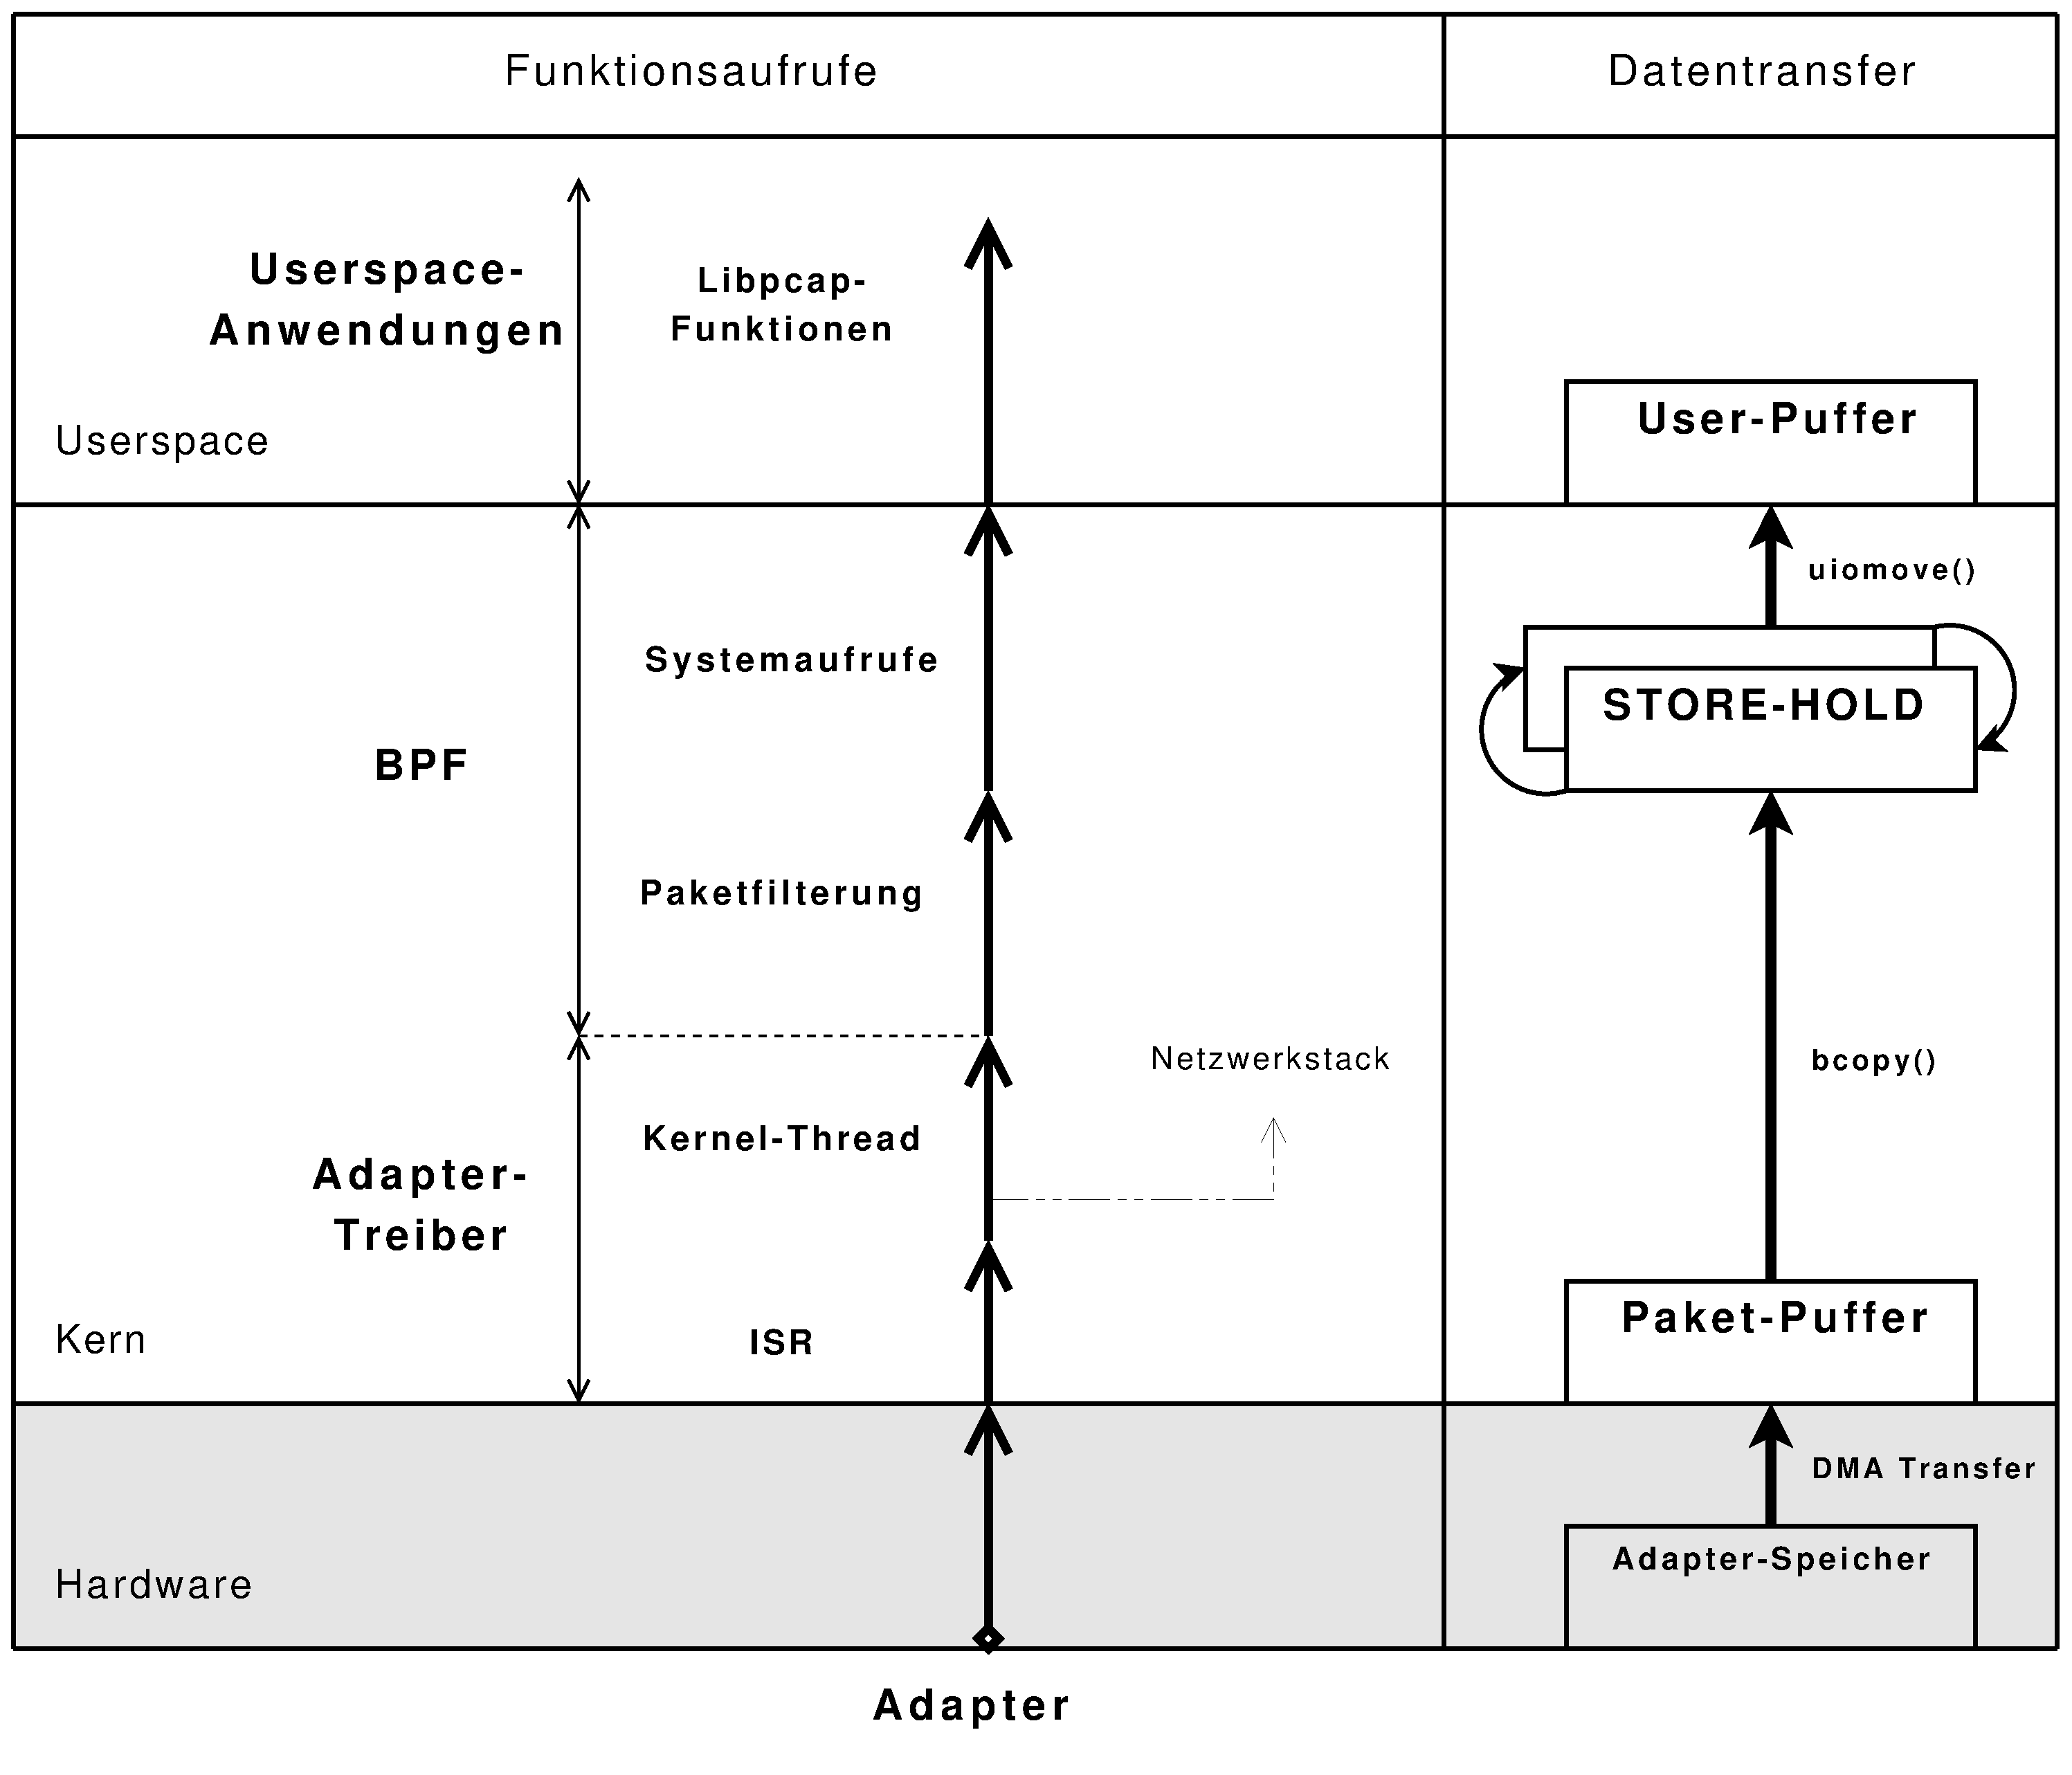
\includegraphics[width=5.1in]{bilder/3copy}
\caption{FreeBSD Packet Capturing Stack}
\label{bsd_cap_stack}
\end{figure}
%
\subsubsection{Interruptbehandlung}\label{sec:intr_behandlung}
Die erste Komponente des Packet-Capturing Stacks (siehe Abbildung
\ref{bsd_cap_stack}) ist der Netzwerk-Treiber. Für jedes empfangene Packet wird
beim Treiber einen neuen Paket-Puffer im RAM alloziert. Nachdem ein Paket vom
Netzwerk-Adapter in den Paket-Puffer kopiert wurde, meldet der Adapter
die Anwesenheit von neuen Daten im RAM durch ein Interrupt, und verursacht damit den
Aufruf der \emph{Interrupt-Service-Routine} (ISR).\\\\ 
%
Da die Interruptbehandlung mit der höchste Priorität ausgeführt wird, sind alle
derzeit laufenden Prozesse auf der aktuellen CPU unterbrochen. Dies kann das
Capturing-Performance negativ beeinflussen, wenn die Interruptbehandlung zu
große  Ausführungszeit hat. Die andere Software-Komponenten, die auf die
empfangene Pakete zugreifen wollen, können in dem Fall nicht genügend
CPU-Zyklen bekommen, denn sie mit der geringeren Priorität ausgeführt sind.
Dies kann zu den vollen Paket-Puffer und als Ergebnis zu den Paketverlusten
führen~\cite{elim_recv_lock}. Deshalb ist es für die Vermeidung von
Paketverlusten sehr wichtig, dass die Interruptbehandlung-Funktionen effizient
implementiert sind und dadurch möglichst kurze Ausführungszeiten haben.\\\\
%
Die Interruptbehandlung wird in zwei Phasen ausgeführt: die eigentliche ISR und
\emph{delayed-ISR}. Die ISR dient nur zum Herausfinden der Ursache des
Interrupts und Planen der delayed-ISR. Die größte Rechenaufwand bei der
Interruptbehandlung findet während der Ausführung des \emph{delayed-ISR}
(Kernel-Thread) statt. Von allen Aufgaben, die der \emph{delayed-ISR} erledigt,
sind die Speicher-Allozierungen, wahrscheinlich, diejenigen die den Großteil
der CPU-Zeit beanspruchen. Während des Paket-Empfangs wird im Kontext von
\emph{delayed-ISR} für jedes empfangene Paket einen neuen Paket-Puffer
alloziert. Dies rettet die bevor empfangene Pakete von Überschreibung hat aber
einen Nachteil, der sich in Vergrößerung des pro-Paket Overhead zeigt,
denn Speicherallozierung ist relativ ``teure'' Operation.
%
\ifthenelse{\boolean{BRIEF}}{}{
%
\begin{figure}
\centering 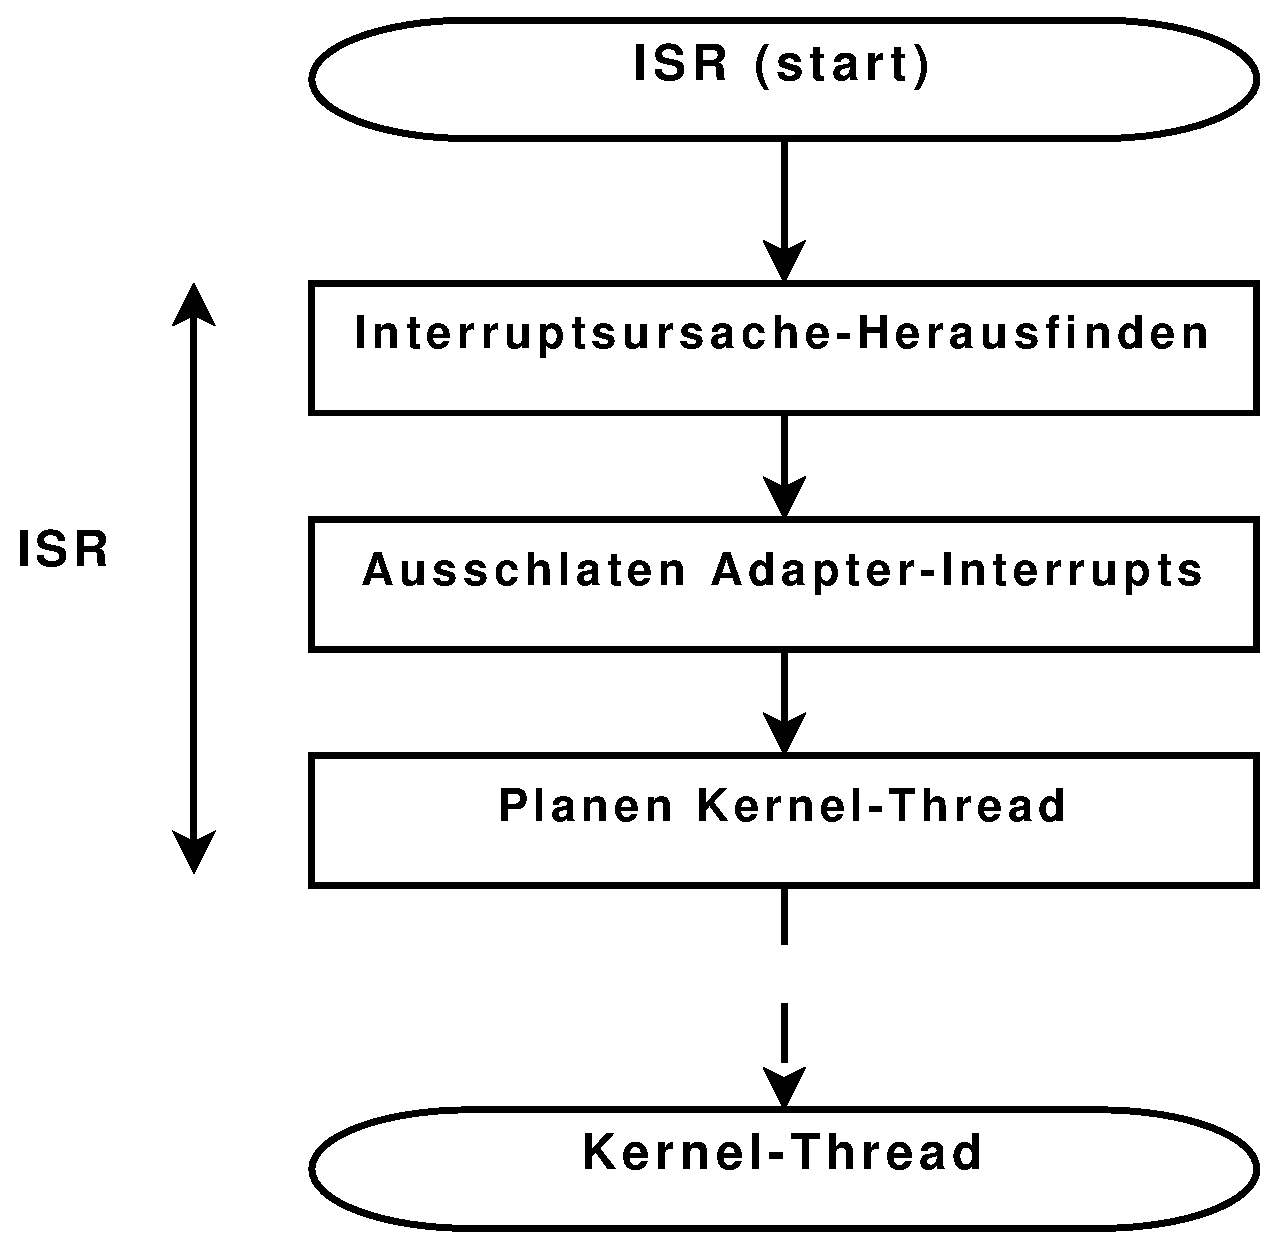
\includegraphics[width=2.0in]{bilder/FlowChart_ISR}
\caption{Adapter-Treiber: Interrupt Service Routine}
\label{img:isr_treiber}
\end{figure}
%
\subsubsection*{Trennung des Interrupt-Handlers in zwei Teile: ISR und Kernel-Thread}\label{sec:intr_isr_kthr}
Da es nicht immer möglich ist, die Ausführungszeit einer ISR zu minimieren,
kann man in ~FreeBSD den Interrupthandler in zwei Teile trennen
~\cite{freebsd_design}.  Der erste Teil ist die eigentliche ISR\footnote{Wird
auch oft in der Literatur als \emph{Fast Interrupt handler} oder \emph{top-half
of interrupt} genannt~\cite{ldd_book}.}, deren Ausführung das Sperren aller
anderen Aktivitäten auf der aktuellen CPU verursacht. Der andere Teil ist ein
Kernel-Thread\footnote{wird auch als \emph{NON-Fast Interrupt handler} oder
\emph{down-half of interrupt} genannt~\cite{ldd_book}.}, dessen Ausführung mit  etwas
niedrigerer Priorität zu einem späteren Zeitpunkt stattfindet (siehe Abbildung
\ref{img:isr_treiber}).\\\\
%
Die ISR des \textbf{em}-Treibers hat  lediglich die Aufgabe durch das Lesen des
\verb+Interrupt-Cause+-Registers (\verb+ICR+)~\cite{e1000_sdm} die Interrupt-Ursache herauszufinden,
die Interrupts des Adapters auszuschalten und die Ausführung eines Kernel-Threads
für die weitere Paketbearbeitung zu planen(siehe Abbildung
\ref{img:isr_treiber}).\\\\
%
Die Aufgabe des Kernel-Threads ist es, die neue durch DMA in die Paket-Puffer
geschrieben Pakete zu lesen, diese auf Fehler zu prüfen, in
\verb+mbuf+-Strukturen~\cite{man_kernel_mbuf, freebsd_design} einzupacken und
dem Protokoll-Stack und BPF zu übergeben (siehe Abbildung
\ref{img:isr_kern_thr}).  Der Kernel-Thread bearbeitet maximal eine bestimmte
Anzahl von Paket-Puffern. Dieser Wert kann über \emph{sysctl}-Befehl
folgender massen gesetzt werden: 
\begin{equation}
			\verb+# sysctl dev.em.0.rx_processing_limit 100+
\end{equation}
Wenn es nach dem Interrupt mehr als \verb+rx_processing_limit+ neue
Paket-Puffer im RAM gibt, wird Kernel-Thread mehrmals geplant. Während des
ersten Ablaufs des Threads sind die Interrupts des Adapter noch gesperrt.  Nach
seinem Ablauf entsperrt der Kernel-Thread die Adapter-Interrupts, sodass die
restlichen Thread-Abläufe mit erlaubten Interrupts stattfinden
und jeder Zeit von neuen
Adapter-Interrupts unterbrochen werden können. Der Grund des Sperrens der
Interrupts nur für den ersten Thread-Ablauf ist nirgendwo beschrieben. Ich
vermute, dass es für dieses Vorgehen folgende Erklärungen gibt: 
\begin{itemize}
	\item Wenn die Interrupts für alle Thread-Abläufe gesperrt wären, könnte
		dann zu lange Inter-Interrupt-Verzögerung entstehen was, den
		Paketverlusten führen würde.
	\item Hätte man vor begin der ersten Thread-Ablauf die Interrupts
		entsperrt, dann könnte bei einer zu hohen Interrupt-Rate dazu kommen, dass der
		Thread ständig durch neue Interrupts unterbrochen würde und dadurch
		nie seine Arbeit erledigt hätte.
\end{itemize}
%
Die Arbeit, die der Kernel-Thread pro Puffer erledigt besteht aus (siehe auch
Abbildung \ref{img:isr_kern_thr}): 
\begin{enumerate}
	\item Allozieren des neuen Paket-Puffer für den aktuellen Deskriptor
	      % \reviewnote{Nenn es eine Variable: P'}
	\item Fehlerprüfung des Paketes im alten Paket-Puffer % \reviewnote{neuer? alter?}
	\item Einpacken des Paketes in \verb+mbuf+-Struktur	
	\item Übergeben des Paketes an den Protokoll-Stack
	\item Übergeben des Paketes an den BPF
	\item Inkrementieren des Wertes in RDT-Register:
		\begin{equation}
			RDT=(RDT+1)\ mod\ SIZE
			\label{form:rdt_inkr}
		\end{equation}
		\emph{SIZE} - Anzahl von Deskriptoren.
\end{enumerate}
\begin{figure}
\centering 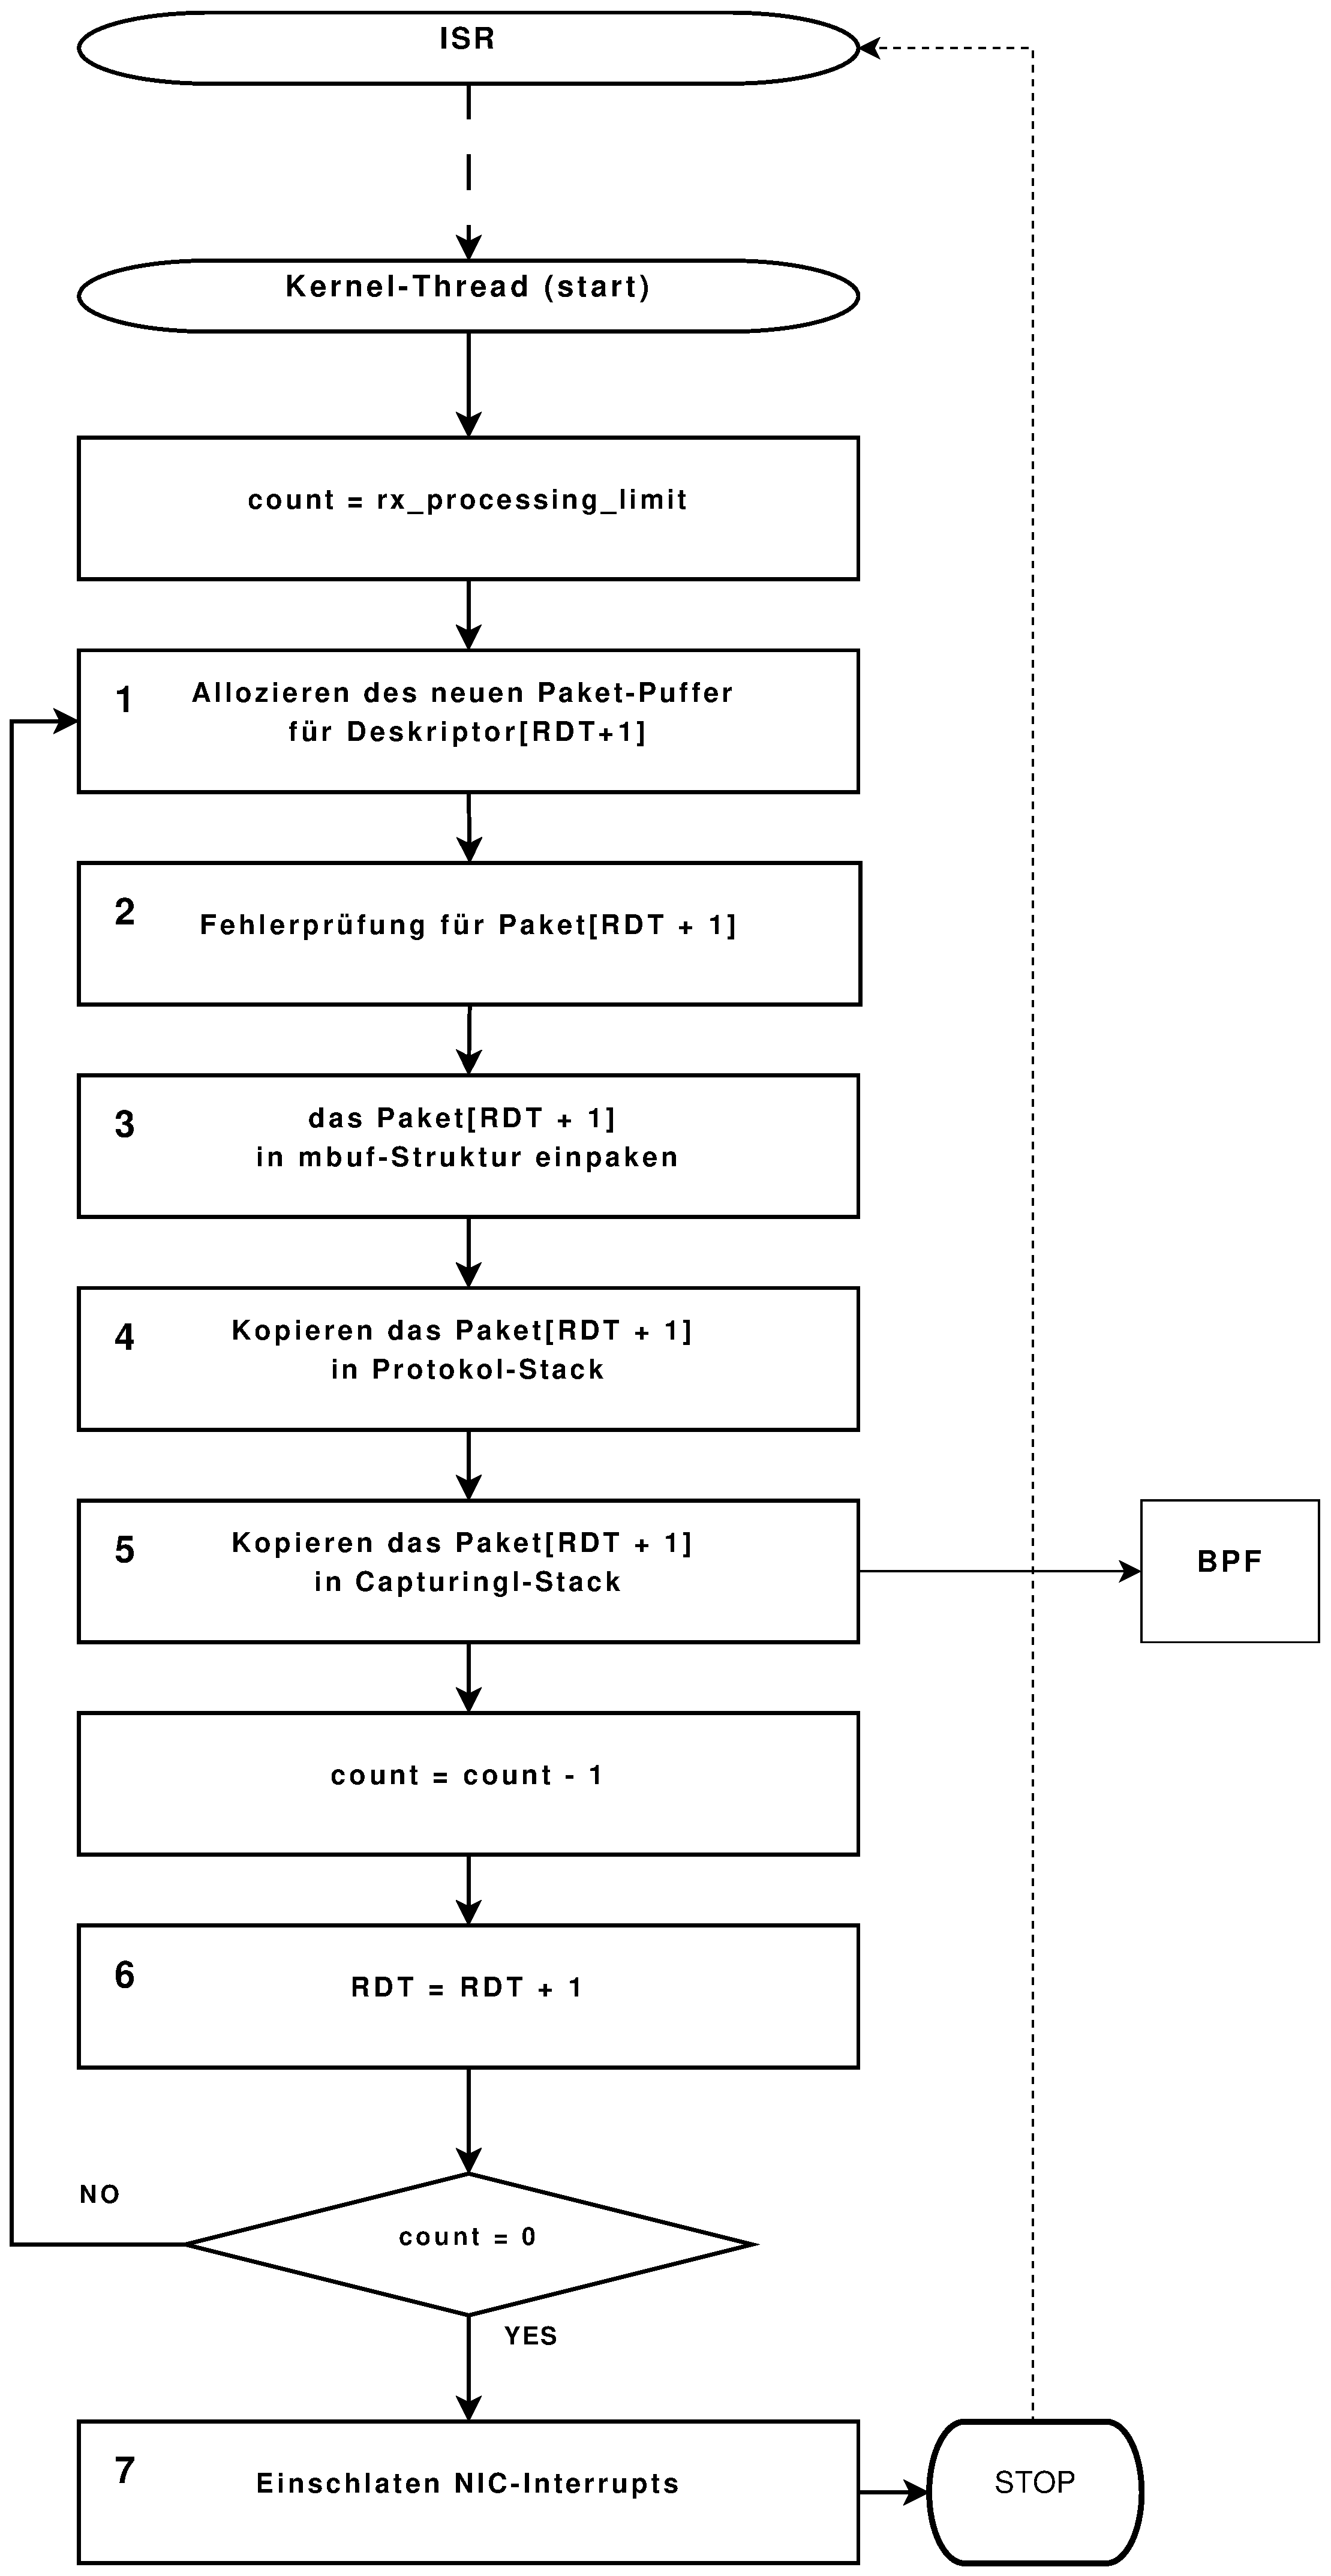
\includegraphics[width=4.5in]{bilder/FlowChart_Kernel_Thread}
\caption{Adapter-Treiber: Kernel-Thread}
\label{img:isr_kern_thr}
\end{figure} 

}
%
\subsubsection{Berkley Packet Filter}\label{sec:bpf}
Der BPF ist die nächste Komponente des FreeBSD Packet-Capturing-Stacks. Der BPF
registriert im System für jeden Prozess, der die Pakete erfassen will ein
symbolisches Device: \verb+/dev/bpf[0-9]+, und bietet dazu eine Menge von
Systemaufrufen (read, ioctl, etc\ldots) für den Zugriff auf die Pakete und zur
Steuerung der Paketfilterung.  Außerdem stellt BPF eine Menge von
Kernel-Funktionen zur Verfügung, die aus dem Treiber aufgerufen werden und die
eigentliche Filterung und Weiterleitung des Paketes durch Capturing-Stack zum
User-Prozess ausführen~\cite{man_kernel_bpf, man_bpf, bpf_paper}.\\\\
%
Die Pakete werden vom BPF gefiltert, und diejenigen, die durch die Filterregeln
akzeptiert wurden, werden in den STORE-HOLD-Puffer kopiert (siehe Abbildung
\ref{bsd_cap_stack}).  Aus dem STORE-HOLD-Puffer werden die Pakete durch den
\emph{read}-Systemaufruf in Userspace übertragen\footnote{Die genaue Beschreibung
ist in \emph{bpf(9)} Manual~\cite{man_kernel_bpf} und in den Papers von Fabian
Schneider~\cite{fabian_da, pcin10gb_paper} zu finden.}.\\\\
%
Der BPF wird auf dem aktuellen FreeBSD vollkommen in Kernelspace ausgeführt.
Es gibt aber auch in der Libpcap-Library eine BPF-Implementierung, was  die
Paketfilterung auch im Userspace erlaubt. Aber das Ausführen von
Filterung-Routinen im Kern, sofort nach dem Paketempfang, hat seine Vorteile.
Die Kopier-Operationen haben mit dem Unterschied zu den anderen wesentlich
längere Ausführungszeiten. Deshalb eliminiert das möglichst frühe Ausführen der
Filterung  das unnötiges Kopieren von Daten, die anhand der vorhandenen
Filterregeln nicht akzeptiert wurden.\\\\
%
Der Performance-Nachteil des klassischen BPF-Models besteht darin, dass es die
``teure'' Paket-Kopier-Operationen im Kernelspace hat und für den Übertragung
der Pakete in den Userspace die Systemaufrufe anfordert, was eine
Kopier-Operation mit dem Ausführung-Kontextwechsel beeinflusst.

\subsubsection{Libpcap}\label{sec:libpcap}
Libpcap ist eine Programm-Bibliothek, die eine Menge von Funktionen zum
bequemen Zugriff auf empfangene Pakete anbietet~\cite{man_pcap}. Mehrere
bekannte Sniffer wie \emph{tcpdump} oder \emph{Wireshark} benutzen Libpcap für
Packet-Capturing.  Auf FreeBSD benutzen die Libpcap-Funktionen  selber
BPF-Systemaufrufe für die Paketfilterung und für Zugriff auf gefilterte Pakete,
und stellen den User-Anwendungen eine bequeme und einfache Schnittstelle für
Capturing.\\\\
%
Während Packet-Capturing sind die Aufgaben der Libpcap-Funktionen, die Pakete in den
Userspace zu holen und den Anwendungen, die auf die Pakete zugreifen wollen einen
Pointer auf Paketpuffer zu übergeben. Dabei besteht keinen großen Overhead, der 
sich deutlich reduzieren lässt. 


\subsection{Namenskonventionen}
Um die Unverständlichkeiten mit den Bezeichnungen zu vermeiden, geben wir 
hier die Namen, unter denen die standard FreeBSD-Capturing-Stack und 
der neuen im Rahmen des Projektes entwickelten Capturing-Stack in den 
weiteren abschnitten auftauchen werden: 
\begin{description}
	\item[ringmap:] Wird als Bezeichnung für die im Rahmen des Projektes 
		entwickelte Capturing-Software benutzt. 
	\item [generic:] Wird als Bezeichnung für die FreeBSD Standard-Capturing-Software benutzt.
\end{description}

\subsection{Zusammenfassung}\label{sec:aufgstel}
In den vorherigen Abschnitten wurden die für Capturing-Performance relevanten
Software-Eigenschaften dargestellt. Dabei wurde versucht herauszufinden, welche
der vorgestellten Komponenten unter welchen Umständen die Performance des
Capturing negativ beeinflussen können. Anhand der herausgefundenen Problemen
werden die konkrete Anforderungen für den Entwurf der neuen Capturing-Software
im Kapitel~\ref{sec:anf_for_entwurf} gestellt.
%
\ifthenelse{\boolean{BRIEF}}{}{
Die Hardware-Komponenten eines Capturing-Systems stellen die höchste
theoretische Grenze für die Capturing-Performance dar. Wir haben aber gesehen, dass
in der Realität die Performance bei der Datenbearbeitung wesentlich schlechter
als die theoretischen Werte sein kann. Das kann man z.B. besonders gut beim
Vergleich der theoretischen~\cite{lodb_wiki} und
effektiven~\cite{steram_results_for_pc} Speicher-Bandbreiten sehen.  Einer der
Gründen dafür ist es, das die Software ineffizient die zur Verfügung stehenden
Hardware-Ressourcen nutzt.\\\\ 
%
Aufgrund der Unmöglichkeit der Verbesserung von Hardware-Komponenten im Rahmen 
einer Diplomarbeit und einer relativen Einfachheit der Software-Lösungen 
hat sich für den praktischen Teil der Diplomarbeit die Softwarebasierende 
Lösung entwickelt. Wir wollen einen neuen Paket-Capturing-Stack implementieren, 
in dem möglichst alle in dem aktuellen Stack gefundene Performance-Probleme 
eliminiert werden.\\\\
%
For allem handelt es sich um die Eliminierung der Kopie-Operationen und
Beseitigung des Systemaufrufes für den Datenzugriff, denn genau diese
Funktionen sind es, die im Vergleich zu den anderen Funktionen, eine relativ große
Ausführungszeit anfordern. Das kann mit dem Memory-Mapping gemacht werden.
Dafür muss aber einen Konzept für den Zugriff auf Daten,  die im ``gemappten''
Puffer liegen, erarbeitet werden.
\subsubsection{Capturing-Stack-Analyse}
}
%
\\\\
Betrachten wir noch mal den in Abbildung~\ref{bsd_cap_stack} dargestellten
Capturing-Stack des aktuellen FreeBSD. Stellen wir uns den Fall vor, wenn alle
Pakete durch die BPF-Filterung akzeptiert sind. Dann gibt es pro Paket drei
Kopier-Operationen:
\begin{enumerate}
\item DMA Transfer in den RAM
	\begin{itemize}
		\item ist mit Hilfe der Hardware erledigt
	\end{itemize}
\item Kopieren in STORE-HOLD-Puffer
	\begin{itemize}
		\item ist mit Hilfe der Kernelfunktion \verb+bcopy(9)+ gemacht. 
	\end{itemize}
\item Kopieren in Userspace
	\begin{itemize}
		\item ist durch den Systemaufruf \emph{read(2)} erledigt, und verursacht damit
			ein Ausführungskontext-Wechsel
	\end{itemize}
\end{enumerate}
Die erste Kopier-Operation, die durch DMA-Transfer erledigt wird, ist
unvermeidlich und nicht optimierbar\footnote{Eigentlich lässt sich der
DMA-Transfer der Paket-Daten in den RAM durch bestimmte Interrupt-Moderation
Einstellungen begrenzt optimieren~\cite{e1000_sdm}}. Aber die restlichen zwei
Kopier-Operationen, ständiges Speicherallozierung für jedes neue Paket und der
Kontext-Wechsel stellen ein Flaschenhals im Capturing-System, falls die Rate
der ankommenden Pakete nah zu $1GBit/sec$ oder höher steigt (siehe Abschnitt
\ref{sec:test_ergebnisse}~Ergebnisse).\\\\
%
Die Kopier-Operationen lassen sich durch die Memory-Mapping eliminieren. Wenn
die Paket-Puffer in den Address-Raum einer Capturing-Anwendung eingeblendet
werden, dann braucht diese Anwendung keine Kopier-Operationen und keine
Systemaufrufe mehr, um auf die Pakete zugreifen zu können. Dafür muss aber ein
Synchronisation-Verfahren erarbeitet werden, wenn die mehrere Prozesse auf den
gleichen Paket-Puffer zugreifen werden.\\\\
%
Die Speicherallozierungen lassen sich durch die Anwendung von dem Ring-Buffer
ersetzen. Der Ring-Buffer präsentiert eine constante Menge der preallozierten
Speicherbereichen und zwei Zeiger: \emph{HEAD} and \emph{TAIL}. Das Besondere am
Ring-Buffer ist es, dass er eine feste Größe hat und die Speicherbereiche die er
verwaltet, nur ein mal alloziert und dann ein nach einander beschrieben und
gelesen werden. Dabei, zeigt \emph{HEAD} auf den nächsten freien
Speicherbereich, der beschrieben wird. \emph{TAIL} zeigt auf den zuletzt
gelesenen Bereich. Im Unterschied zum normalen Array werden die ältesten Inhalte
überschrieben, wenn der Ring-Buffer voll ist und weitere Elemente abgelegt werden.
%

\newpage
\ifthenelse{\boolean{BRIEF}}{
\section{Anforderungen für den neuen Capturing-Stack}\label{sec:anf_for_entwurf}
}{
\subsubsection{Anforderungen für den Entwurf}\label{sec:anf_for_entwurf}
}
\subsection{Eliminierung der Kopier-Operationen}
Die zwei Paket-Kopie-Operationen, vom Paket-Puffer in den BPF-Puffer und vom
BPF-Puffer in den Puffer des Userspace-Anwendung, sollen eliminiert werden
(Abbildung \ref{img:new_stack}) Die Pakete sollen sofort nach dem DMA-Transfer
im virtuellen Speicher des User-Capturing-Prozesses zugreifbar sein. Dafür
sollen die Paket-Puffer in den Adressraum der Capturing-Anwendung eingeblendet
werden. Das entsprechende Synchronisationssverfahren muss für den Zugriff auf 
Paket-Puffer und auf $HEAD/TAIL$-Pointers erarbeitet werden.
%
\subsection{Eliminierung der Speicherallozierungen}
Keine neue Paket-Puffer sollen für die neue ankommende Pakete alloziert werden. 
Alle Speicherbereiche für die Pakete und \emph{mbuf}'s sollen als Ring-Buffer 
verwaltet werden. Die ältere Inhalte sollen mit den neuen Daten überschrieben 
werden, wenn der Ring-Buffer voll ist. 
\subsection{Keine Systemaufrufe für den Zugriff auf Pakete}
Es sollen möglichst keine Systemaufrufe während Capturing auftreten, denn die
Systemaufrufe verursachen den Ausführungs-Kontextwechsel, was relativ zu den
anderen Operationen, eine sehr große Menge von System-Ressourcen anfordert.
		\begin{itemize}
			\item Dafür müssen außer den Paket-Puffern noch andere
				Datenstrukturen mit den für das Capturing relevanten Daten in den
				Userspace eingeblendet werden, damit der User-Prozess ohne
				Systemaufrufe die Daten vom Treiber bekommt und auch
				Informationen an den Treiber liefern und damit das Capturing
				steuern kann.
			\item   Systemaufrufe sind nur während der Initialisierung des
				Capturing-Prozesses 
			        % versteh ich nicht, kann auch weg, oder? -- Andi
			        %für das Holen der benötigten Daten vom
				%Adapter in den Userspace,
				und während der Abwesenheit von neuen
				Paketen für das Blockieren des auf die Pakete wartenden
				Prozesses erlaubt. 
		\end{itemize}
\subsection{Eine Userspace-Capturing-Anwendung pro Netzwerk-Interface}
Wir begrenzen uns auf nur eine gleichzeitig aktive
Userspace-Capturing-Anwendung pro Netzwerk-Interface, um den Entwurf und die
Implementierung einfach zu halten. Außerdem, die Vergrösserung der Menge der
Anwendungen, welche von dem gleichen Interface die Pakete erfassen, erhöht
nicht die Capturing-Performance\footnote{Mit der Ausnahme eines Multi-queue
Controllers, wenn es mehrere Anwendungen parallel, eine Anwendung per
receive-queue, ausgeführt werden}

\subsection{Transparenz}
Die Funktionalität des neuen Capturing-Stacks soll für die standard Anwendungen
möglichst unsichtbar sein. Das heißt, die standard Funktionen des
Netzwerktreibers, Protokoll-Stacks, BPF's sollen nicht durch die Anwesenheit
von \emph{ringmap} gestört werden. In einem \emph{default} Zustand sollen die
standard Funktionen des Betriebssystem aktiviert werden.  Das Aktivieren des
\emph{ringmap} soll z.B. über ein Systemaufruf realisiert werden. Dabei im
\emph{ringmap}-Modus können Protokoll-Stack und standard Packet-Capturing-Stack
deaktiviert werden. Das zurücksetzen des System in den default-Mode soll auch
ohne Rekompilation und ohne System-Neustart möglich sein.\\\\
%
Standard-FreeBSD-Capturing-Stack die empfangene Pakete den Userspace-Prozessen
zur Verfügung stellt, müssen die Userspace-Prozesse anders auf die Pakete
zugreifen. Um der neue Stack einsetzbar zu machen soll am besten die
Libpcap-Library für ihn angepasst werden, sodass für alle
Capturing-Anwendungen, die auf Libpcap basieren, keine Änderungen benötigt
werden. 

\begin{figure}
	\begin{center}
	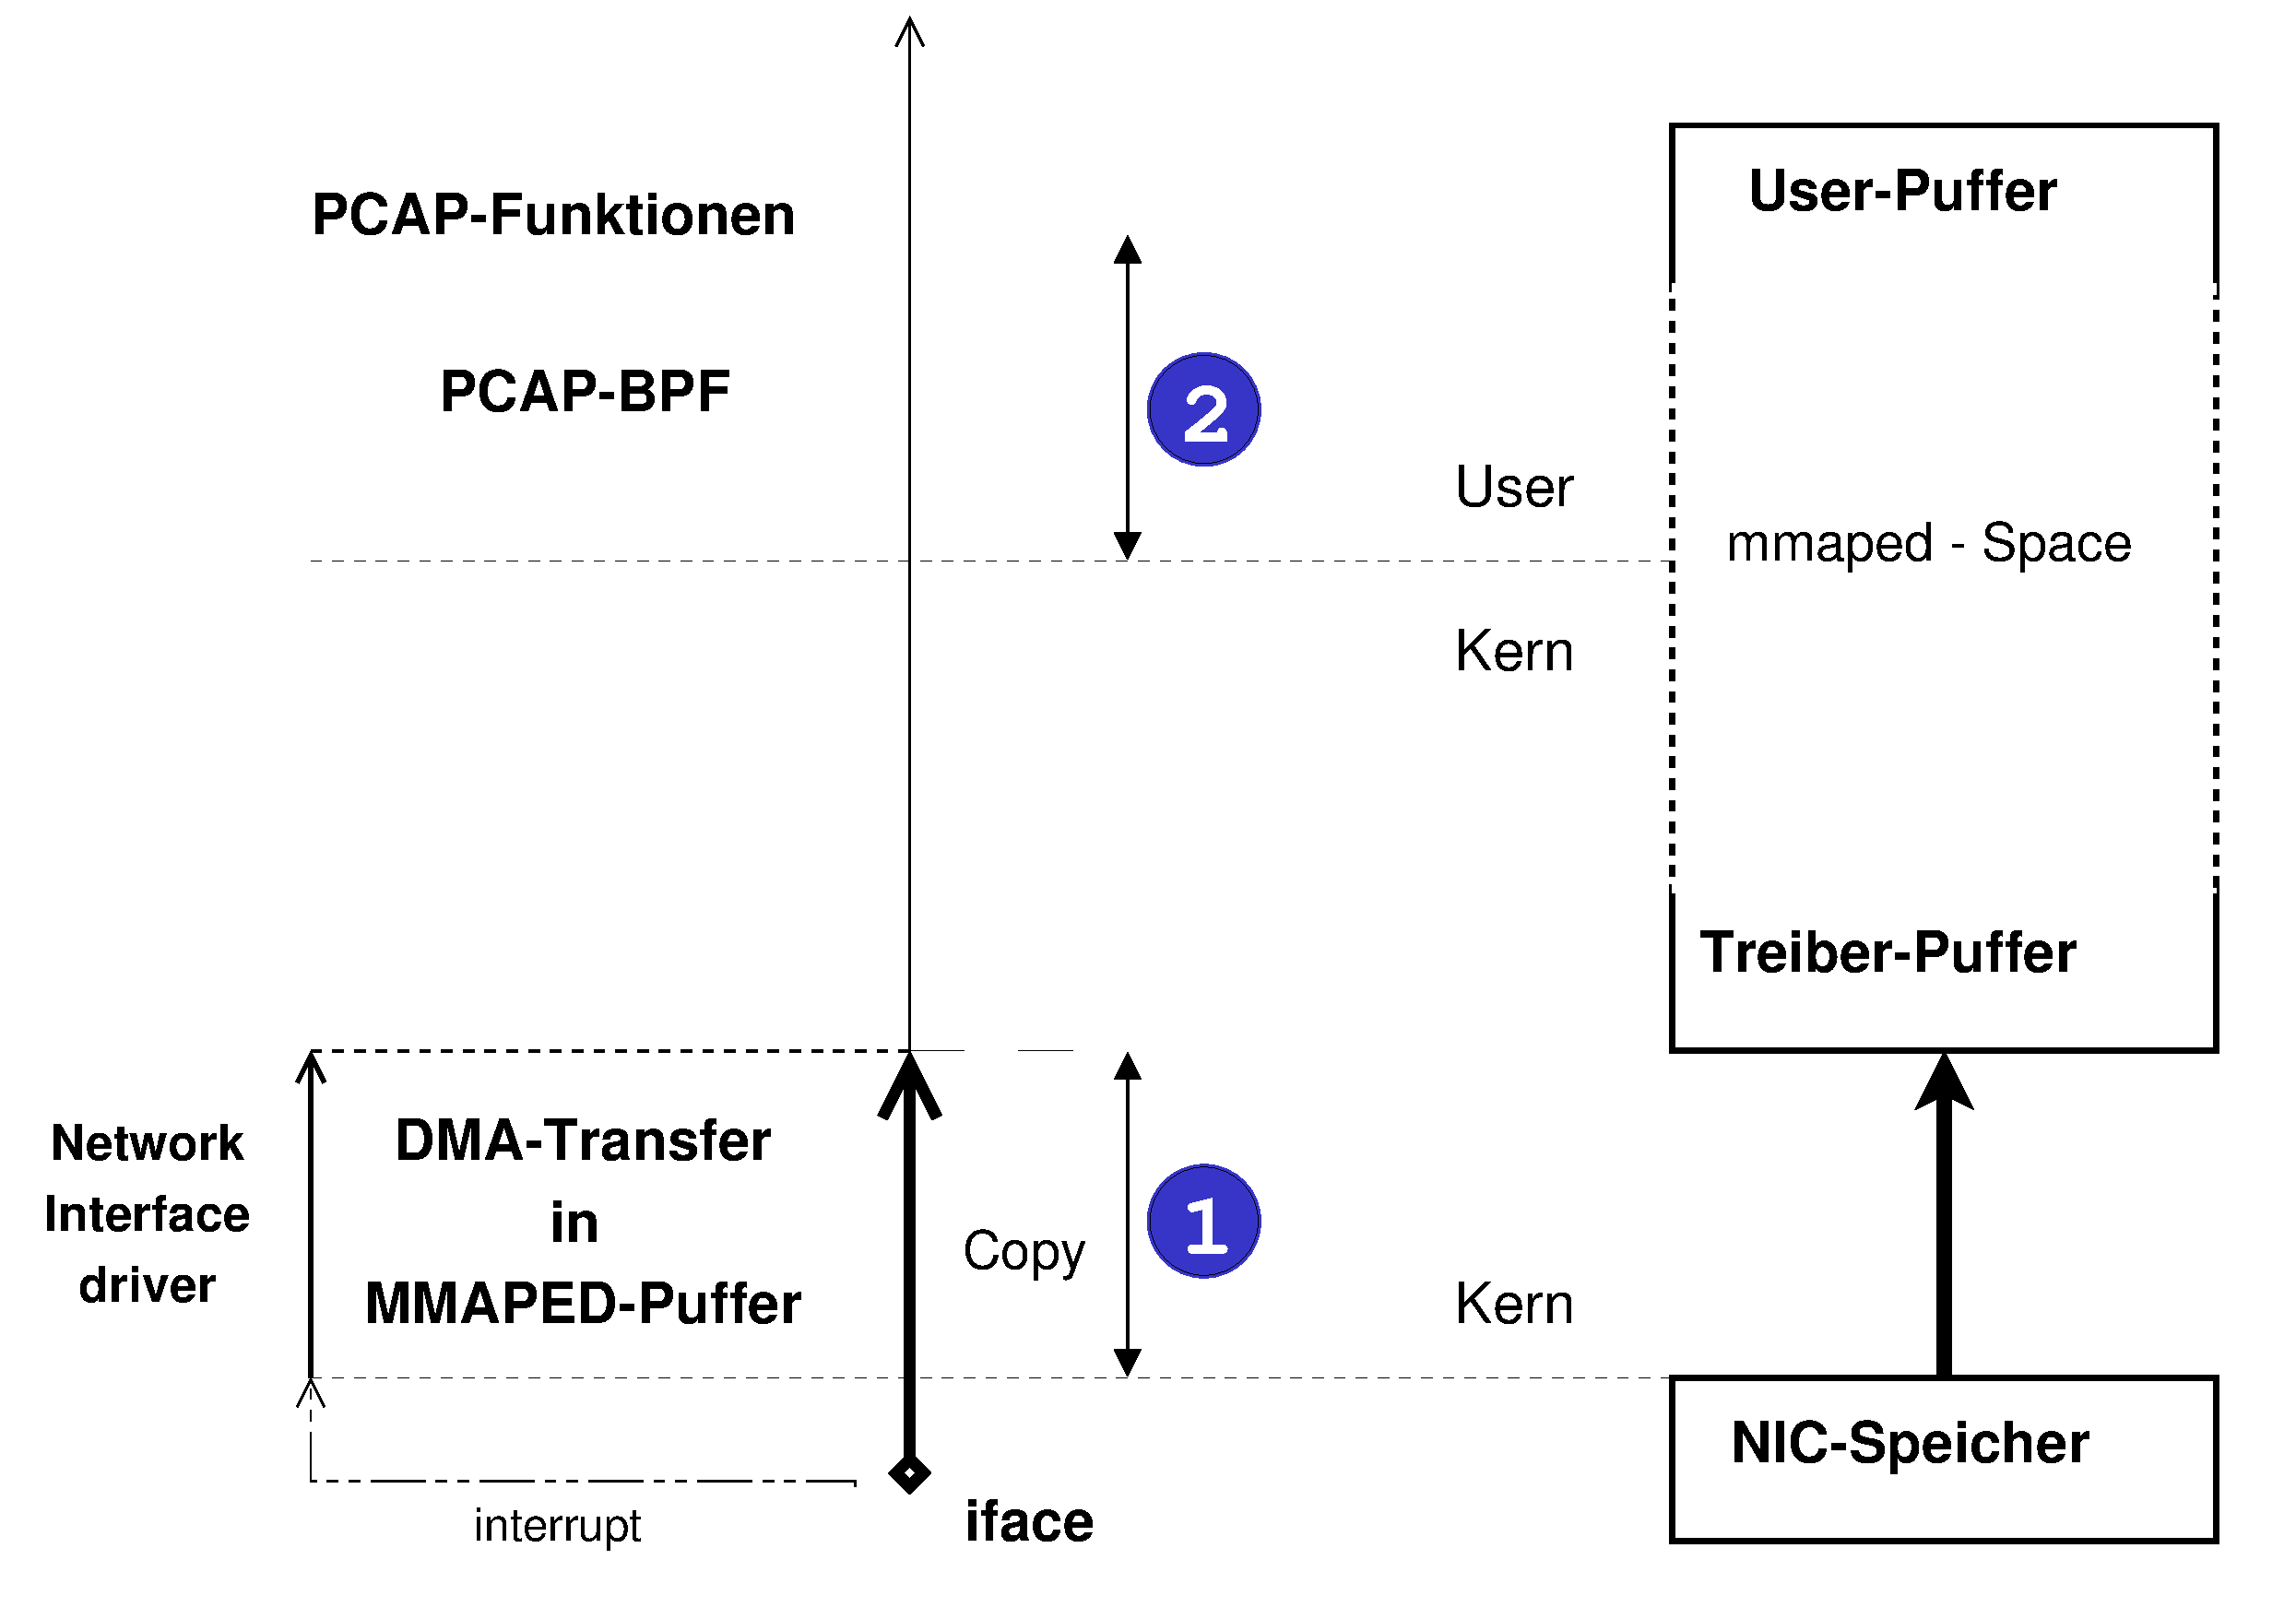
\includegraphics[width=4.9in]{bilder/1copy}
	\end{center}
	\caption{Der neue ringmap-Capturing-Stack. Ziel des Projektes}
	\label{img:new_stack}
\end{figure}

\ifthenelse{\boolean{BRIEF}}{}{
\subsection{Zusammenfassung}
In diesem Kapitel wurden die für das Verständnis der Capturing-Problematik
relevanten Hintergründe dargestellt. Es wurden sowohl die Software- als auch
die Hardware-Aspekte, welche die Capturing-Performance beeinflussen können,
betrachtet und analysiert. Die Hardware-Eigenschaften eines Capturing-System
sind deshalb wichtig, weil für die Diplomarbeit eine konkrete  Hardware
vorausgesetzt wurde (siehe Abschnitt \ref{sec:hwsw_voraus}), und die
Problemlösung für das Erreichen der maximalen Capturing-Performance
Hardware-Abhängig sein dürfte.\\\\
Außerdem es wurden einige Hardware-Eigenschaften erläutert die zwar keinen
Einfluss auf die Implementierung des neuen Paket-Capturing-Stack haben, 
aber vom Benutzer des Betriebssystem geändert werden können und dadurch die
Capturing-Performance beeinflussen. Es handelt sich dabei um
\emph{Interrupt-Coalescing} (Abschnitt \ref{sec:intr_coal}) und
\emph{Prozessoraffinität} (Abschnitt \ref{sec:cpu_einfl_auf_cap}). Die
Notwendigkeit diese Eigenschaften zu kennen liegt darin, dass sie unabhängig
von Effizienz der Implementierung der Capturing-Software die
Capturing-Performance beeinflussen und dadurch bei ungünstigen Einstellungen
reduzieren können.\\\\
%
Beim Betrachten der unterschiedlichen Hardware- und Software-Komponenten wurde
auch analysiert unter welchen Umständen Engstellen beim Capturing auftreten
können, und anhand der herausgestellten Problemen wurden die Anforderungen für
den praktischen Teil der Diplomarbeit definiert (Abschnitt
\ref{sec:aufgstel}).\\\\ 
%
Das Ziel des praktischen Teiles der Diplomarbeit ist die Implementierung eines
neuen Capturing-Stacks für das Betriebssystem FreeBSD. Dafür soll eine neue
Software implementiert werden, deren Aufgaben es ist, die gefundenen
Engstellen, die bei der Bearbeitung der im RAM liegenden Pakete entstehen
können, zu beseitigen. Es handelt sich vor allem um die Kopier-Operationen und
die Systemaufrufe, die bei Paket-Filterung oder beim Paket-Zugriff verwendet
werden. \\\\
%
Die Capturing-Performance-Probleme die während der Speicherung der Pakete auf
die Festplatte und der Darstellung der Pakete auf dem Terminal auftreten können wurden nicht
Betrachtet und sind nicht Gegenstand dieser Arbeit.
}
